\documentclass{article}
\usepackage[UTF8]{ctex} % 用于中文排版
\usepackage{geometry}
\usepackage{indentfirst}
\usepackage{enumitem}

\usepackage{titling}    % 用于自定义标题页
\usepackage{graphicx}
\usepackage{float}

\usepackage{xcolor}
\usepackage{listings}

\usepackage{setspace}

% 页面几何设置
\geometry{a4paper, left=25mm, right=25mm, top=25mm, bottom=25mm}
% 取消首行缩进
\setlength{\parindent}{0pt}
% 行间距设置
\setstretch{1.5}
% 自定义字体大小
\newcommand{\fourhao}{\fontsize{14pt}{\baselineskip}\selectfont} % 四号字体
\newcommand{\xiaosihao}{\fontsize{12pt}{\baselineskip}\selectfont} % 小四号字体
\newcommand{\song}{\CJKfamily{song}}
% 设置代码块格式
\lstset{
    basicstyle = \footnotesize\ttfamily,                 % 设置行距,字体
    numbers = left,                                      % 在左侧显示行号
    numberstyle = \tiny \color{gray},                    % 设定行号格式
    keywordstyle = \bfseries \color[RGB]{40,40,255},     % 设定关键字颜色
    numberstyle = \footnotesize \color{darkgray},           
    commentstyle = \color[RGB]{0,96,96},                 % 设置代码注释的格式
    stringstyle = \color[RGB]{128,0,0},                  % 设置字符串格式
    frame = single,                                      % 不显示背景边框
    backgroundcolor = \color[RGB]{245,245,244},          % 设定背景颜色
    language=Verilog                                     % 设置语言
}
\raggedbottom   % 段落间留白, 避免排版时自动拉伸导致的行间距变化。
\begin{document}

% 封面页面
\begin{titlepage}
    \centering
    \vspace*{2cm}

    \Huge
    \textbf{课程名称:EDA 技术综合设计}

    \vspace{2cm}

    \LARGE
    设计报告名称:设计六\ 整数乘法器

    \vspace{4cm}

    \centering
    \Large
    \begin{tabular}{rl}
        班级: & 通信214    \\
        姓名: & \ 王峤宇    \\
        学号: & \ 214022
    \end{tabular}

    \vfill

    \vspace{1cm}
\end{titlepage}

\newpage
% 第一部分
\section*{\fourhao 一、设计内容及原理}
\xiaosihao
\setstretch{1.5}
% 设计项目内容及设计原理,如真值表、状态表及状态转换图、文字说明等。
\subsection*{基础任务}
\textbf{设计任务}:输入两个无符号四位二进制(BCD 码)整数,求出它们的乘法结果,输入由拨码开关给入,输入输出由数码管十进制显示。\\
二进制的整数乘法可以通过移位累加的方式实现。
\begin{figure}[htbp]
    \centering
    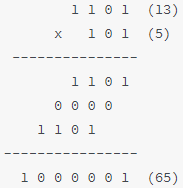
\includegraphics[width=0.3\textwidth]{image/2024-06-20-18-08-28.png}
    \caption{移位累加过程}
    \label{image_design_1}
\end{figure}
二进制整数乘法实现原理如图\ref{image_design_1}所示, 对于BCD码直接相乘, 可以直接视为二进制相乘。
\subsection*{提高内容}
\textbf{设计任务}:输入两个无符号四位二进制(8421 码)整数,求出它们的十进制乘法结果,输入由拨码开关给入,
输入输出由数码管十
进制显示。\\
\subsection*{拓展任务}
\textbf{任务要求}:输入两个无符号二进制整数(16-99 范围即可,也可更大但最大 256,这样输出用 5 位数码管,输入用 3 位数码管,
刚好够用),求出它们的十进制乘法结果,输入由拨码开关给入,用数码管显示输入输出数值。\\

% 第二部分
\section*{\fourhao 二、设计过程}
\xiaosihao
\setstretch{1.5}
% 从工程建立开始,一直到硬件调试。
% 按照基础任务、提高任务和拓展任务分别给出相应的源文件、仿真文件、约束文件
\subsection*{基础任务}
对于BCD码直接相乘的模块设计源文件如下:
\begin{lstlisting}[language=Verilog, caption={4位BCD码相乘}]
/* 四位bcd乘法器 */
module mult_bcd(
    input clk,              /* 时钟 */
    input rst,              /* 异步高电平复位 */
    input data_in_rdy,      /* 输入数据有效 */
    input [3:0] bcd_in_1,   /* 输入乘数 */
    input [3:0] bcd_in_2,   /* 输入被乘数 */
    output data_out_rdy,    /* 输出数据有效 */
    output [3:0] bcd_out_1, /* 输出结果高位 */
    output [3:0] bcd_out_2  /* 输出结果低位 */
    );
    reg [1:0] cnt;
    always @(posedge clk or posedge rst) begin
        if (rst) begin
            cnt <= 2'b0;
        end
        else if (data_in_rdy) begin
            cnt <= cnt + 1'b1;
        end
        else begin
            cnt <= 2'b0;
        end
    end

    reg [7:0] num1;
    reg [3:0] num2;
    reg [7:0] acc;
    /* 累加求解乘法 */
    always @(posedge clk or posedge rst) begin
        if (rst) begin
            acc <= 8'b0;
            num1 <= 8'b0;
            num2 <= 4'b0;
        end
        else if (data_in_rdy && cnt == 2'b0) begin
            num1 <= bcd_in_1 << 1;
            num2 <= bcd_in_2 >> 1;
            acc <= bcd_in_2[0] ? bcd_in_1 : 8'b0;
        end
        else if (cnt != 2'd3) begin
            num1 <= num1 << 1;
            num2 <= num2 >> 1;
            acc <= num2[0] ? num1 + acc : acc;
        end
        else begin
            acc <= acc;
        end
    end

    reg [7:0] res;
    reg data_out_rdy_r;
    always @(posedge clk or posedge rst) begin
        if (rst) begin
            data_out_rdy_r <= 1'b0;
            res <= 8'b0;
        end
        else if (cnt == 2'd3) begin
            data_out_rdy_r <= 1'b1;
            res <= acc;
        end
        else begin
            data_out_rdy_r <= 1'b0;
            res <= 8'b0;
        end
    end
    assign data_out_rdy = data_out_rdy_r;

    wire [3:0] bcd_foobar;
    bin2bcd_8bit  bin2bcd_8bit_inst (
        .bin(res),
        .bcd_12bit({bcd_foobar, bcd_out_1, bcd_out_2})
    );
endmodule
\end{lstlisting}
其中二进制转BCD码源文件如下:
\begin{lstlisting}[language=Verilog, caption={二进制转BCD码}]
module bin2bcd_8bit(
    input [7:0] bin, 
    output [11:0] bcd_12bit  /* 高中低BCD结果 */
    );

    integer i;
    reg [19:0] bcd_temp;
    always @(*) begin
        // 初始化, 直接移位三次
        bcd_temp = {9'b0, bin, 3'b0};
        // 逐位移位法
        for (i = 0; i < 5; i = i + 1'b1) begin
            // 如果BCD的每一部分 > 4,加3
            if (bcd_temp[11:8] > 4)
                bcd_temp[11:8] = bcd_temp[11:8] + 3;
            if (bcd_temp[15:12] > 4)
                bcd_temp[15:12] = bcd_temp[15:12] + 3;
            if (bcd_temp[19:16] > 4)
                bcd_temp[19:16] = bcd_temp[19:16] + 3;
            // 左移1位
            bcd_temp = {bcd_temp[18:0], 1'b0};
        end
    end
    assign bcd_12bit = bcd_temp[19-:12];
endmodule
\end{lstlisting}
top文件如下:
\begin{lstlisting}[language=Verilog, caption={top}]
module mult_bcd_top(
    input clk,                      /* 时钟 */
    input rst,                      /* 异步高电平复位 */
    input [7:0] keys,               /* 8个拨码开关输入 */
    input [7:0] dip,                /* dip开关输入 */
    output [7:0] sseg1, sseg2,      /* 八段数码管 */
    output [3:0] an1, an2           /* 数码管片选信号 */
    );

    /* 例化时分复用的乘法器模块 */
    wire [3:0] bcd_out_1;
    wire [3:0] bcd_out_2;
    wire data_out_rdy;
    mult_bcd  mult_bcd_inst (
        .clk(clk),
        .rst(rst),
        .data_in_rdy(1'b1),
        .bcd_in_1(keys[3:0]),
        .bcd_in_2(dip[3:0]),
        .data_out_rdy(data_out_rdy),
        .bcd_out_1(bcd_out_1),
        .bcd_out_2(bcd_out_2)
    );
    /* 第一个数码管显示 */
    reg [3:0] dsp_buffer_1[0:3];
    always @(posedge clk) begin
        dsp_buffer_1[0] <= keys[3:0];
        dsp_buffer_1[1] <= 4'd10;
        dsp_buffer_1[2] <= 4'd10;
        dsp_buffer_1[3] <= dip[3:0];
    end
    /* 第二个数码管显示 */
    reg [3:0] dsp_buffer_2[0:3];
    always @(posedge clk or posedge rst) begin
        if (rst) begin
            dsp_buffer_2[0] <= 4'd10;
            dsp_buffer_2[1] <= 4'd10;
            dsp_buffer_2[2] <= 4'd10;
            dsp_buffer_2[3] <= 4'd10;
        end
        else if (data_out_rdy) begin
            dsp_buffer_2[0] <= 4'd10;
            dsp_buffer_2[1] <= 4'd10;
            dsp_buffer_2[2] <= bcd_out_1;
            dsp_buffer_2[3] <= bcd_out_2;
        end
        else begin
            dsp_buffer_2[0] <= 4'd10;
            dsp_buffer_2[1] <= 4'd10;
            dsp_buffer_2[2] <= dsp_buffer_2[2];
            dsp_buffer_2[3] <= dsp_buffer_2[3];
        end
    end
    /* 第一个四位数码管 */
    scan_led_hex_disp_4  scan_led_hex_disp_4_inst_1 (
        .clk(clk), .rst(rst),
        .hex0(dsp_buffer_1[0]), .hex1(dsp_buffer_1[1]),
        .hex2(dsp_buffer_1[2]), .hex3(dsp_buffer_1[3]),
        .dp(4'b0000), .an(an1), .sseg(sseg1)
    );
    /* 第二个四位数码管 */
    scan_led_hex_disp_4  scan_led_hex_disp_4_inst_2 (
        .clk(clk), .rst(rst),
        .hex0(dsp_buffer_2[0]), .hex1(dsp_buffer_2[1]),
        .hex2(dsp_buffer_2[2]), .hex3(dsp_buffer_2[3]),
        .dp(4'b0000), .an(an2), .sseg(sseg2)
    );
endmodule    
\end{lstlisting}
针对模块的仿真文件如下:
\begin{lstlisting}[language=Verilog, caption={BCD乘法器仿真文件}]
module mult_bcd_tb;
    //Ports
    reg  clk;
    reg  rst;
    reg  data_in_rdy;
    reg [3:0] bcd_in_1;
    reg [3:0] bcd_in_2;
    wire  data_out_rdy;
    wire [3:0] bcd_out_1;
    wire [3:0] bcd_out_2;

    reg [3:0] bcd_res[0:1];
    initial begin
        clk = 0;
        rst = 0;
        #10;
        rst = 1;
        #10;
        rst = 0;
        bcd_in_1 = 4'd4;
        bcd_in_2 = 4'd5;
        data_in_rdy = 1'b1;

        wait(data_out_rdy == 1'b1);
        data_in_rdy = 1'b0;
        bcd_res[0] = bcd_out_1;
        bcd_res[1] = bcd_out_2;
        #20;
        $finish;
    end

    mult_bcd  mult_bcd_inst (
        .clk(clk),
        .rst(rst),
        .data_in_rdy(data_in_rdy),
        .bcd_in_1(bcd_in_1),
        .bcd_in_2(bcd_in_2),
        .data_out_rdy(data_out_rdy),
        .bcd_out_1(bcd_out_1),
        .bcd_out_2(bcd_out_2)
    );

    always #5  clk = ! clk ;
endmodule
\end{lstlisting}
基础任务、调高任务以及拓展任务公用的约束文件如下:
\begin{lstlisting}[language=Verilog, caption={约束文件}]
/* 100MHz时钟信号 */
set_property -dict {PACKAGE_PIN P17 IOSTANDARD LVCMOS33} [get_ports clk]
/* 复位信号 */
set_property -dict {PACKAGE_PIN R11 IOSTANDARD LVCMOS33} [get_ports rst]
/* 拨码开关 */
set_property -dict {PACKAGE_PIN P5 IOSTANDARD LVCMOS33} [get_ports {keys[7]}]
set_property -dict {PACKAGE_PIN P4 IOSTANDARD LVCMOS33} [get_ports {keys[6]}]
set_property -dict {PACKAGE_PIN P3 IOSTANDARD LVCMOS33} [get_ports {keys[5]}]
set_property -dict {PACKAGE_PIN P2 IOSTANDARD LVCMOS33} [get_ports {keys[4]}]
set_property -dict {PACKAGE_PIN R2 IOSTANDARD LVCMOS33} [get_ports {keys[3]}]
set_property -dict {PACKAGE_PIN M4 IOSTANDARD LVCMOS33} [get_ports {keys[2]}]
set_property -dict {PACKAGE_PIN N4 IOSTANDARD LVCMOS33} [get_ports {keys[1]}]
set_property -dict {PACKAGE_PIN R1 IOSTANDARD LVCMOS33} [get_ports {keys[0]}]
/* DIP */
set_property -dict {PACKAGE_PIN U3 IOSTANDARD LVCMOS33} [get_ports {dip[7]}]
set_property -dict {PACKAGE_PIN U2 IOSTANDARD LVCMOS33} [get_ports {dip[6]}]
set_property -dict {PACKAGE_PIN V2 IOSTANDARD LVCMOS33} [get_ports {dip[5]}]
set_property -dict {PACKAGE_PIN V5 IOSTANDARD LVCMOS33} [get_ports {dip[4]}]
set_property -dict {PACKAGE_PIN V4 IOSTANDARD LVCMOS33} [get_ports {dip[3]}]
set_property -dict {PACKAGE_PIN R3 IOSTANDARD LVCMOS33} [get_ports {dip[2]}]
set_property -dict {PACKAGE_PIN T3 IOSTANDARD LVCMOS33} [get_ports {dip[1]}]
set_property -dict {PACKAGE_PIN T5 IOSTANDARD LVCMOS33} [get_ports {dip[0]}]
/* 数码管 */
set_property -dict {PACKAGE_PIN G2 IOSTANDARD LVCMOS33} [get_ports {an1[0]}]
set_property -dict {PACKAGE_PIN C2 IOSTANDARD LVCMOS33} [get_ports {an1[1]}]
set_property -dict {PACKAGE_PIN C1 IOSTANDARD LVCMOS33} [get_ports {an1[2]}]
set_property -dict {PACKAGE_PIN H1 IOSTANDARD LVCMOS33} [get_ports {an1[3]}]
set_property -dict {PACKAGE_PIN G6 IOSTANDARD LVCMOS33} [get_ports {an2[3]}]
set_property -dict {PACKAGE_PIN E1 IOSTANDARD LVCMOS33} [get_ports {an2[2]}]
set_property -dict {PACKAGE_PIN F1 IOSTANDARD LVCMOS33} [get_ports {an2[1]}]
set_property -dict {PACKAGE_PIN G1 IOSTANDARD LVCMOS33} [get_ports {an2[0]}]
set_property -dict {PACKAGE_PIN D5 IOSTANDARD LVCMOS33} [get_ports {sseg1[7]}]
set_property -dict {PACKAGE_PIN B4 IOSTANDARD LVCMOS33} [get_ports {sseg1[6]}]
set_property -dict {PACKAGE_PIN A4 IOSTANDARD LVCMOS33} [get_ports {sseg1[5]}]
set_property -dict {PACKAGE_PIN A3 IOSTANDARD LVCMOS33} [get_ports {sseg1[4]}]
set_property -dict {PACKAGE_PIN B1 IOSTANDARD LVCMOS33} [get_ports {sseg1[3]}]
set_property -dict {PACKAGE_PIN A1 IOSTANDARD LVCMOS33} [get_ports {sseg1[2]}]
set_property -dict {PACKAGE_PIN B3 IOSTANDARD LVCMOS33} [get_ports {sseg1[1]}]
set_property -dict {PACKAGE_PIN B2 IOSTANDARD LVCMOS33} [get_ports {sseg1[0]}]
set_property -dict {PACKAGE_PIN H2 IOSTANDARD LVCMOS33} [get_ports {sseg2[7]}]
set_property -dict {PACKAGE_PIN D4 IOSTANDARD LVCMOS33} [get_ports {sseg2[6]}]
set_property -dict {PACKAGE_PIN E3 IOSTANDARD LVCMOS33} [get_ports {sseg2[5]}]
set_property -dict {PACKAGE_PIN D3 IOSTANDARD LVCMOS33} [get_ports {sseg2[4]}]
set_property -dict {PACKAGE_PIN F4 IOSTANDARD LVCMOS33} [get_ports {sseg2[3]}]
set_property -dict {PACKAGE_PIN F3 IOSTANDARD LVCMOS33} [get_ports {sseg2[2]}]
set_property -dict {PACKAGE_PIN E2 IOSTANDARD LVCMOS33} [get_ports {sseg2[1]}]
set_property -dict {PACKAGE_PIN D2 IOSTANDARD LVCMOS33} [get_ports {sseg2[0]}]
\end{lstlisting}
\subsection*{提高任务}
四位二进制乘法源码如下
\begin{lstlisting}[language=Verilog, caption={四位二进制乘法源码}]
module mult_bin(
    input clk,              /* 时钟 */
    input rst,              /* 异步高电平复位 */
    input data_in_rdy,      /* 输入数据有效 */
    input [7:0] data_in_1,  /* 输入乘数 */
    input [7:0] data_in_2,  /* 输入被乘数 */
    output data_out_rdy,    /* 输出数据有效 */
    output [15:0] data_out  /* 输出8位数据 */        
    );
    reg [2:0] cnt;
    always @(posedge clk or posedge rst) begin
        if (rst) begin
            cnt <= 2'b0;
        end
        else if (data_in_rdy) begin
            cnt <= cnt + 1'b1;
        end
        else begin
            cnt <= 2'b0;
        end
    end

    reg [15:0] num1;
    reg [7:0] num2;
    reg [15:0] acc;
    /* 累加求解乘法 */
    always @(posedge clk or posedge rst) begin
        if (rst) begin
            acc <= 16'b0;
            num1 <= 16'b0;
            num2 <= 8'b0;
        end
        else if (data_in_rdy && cnt == 2'b0) begin
            num1 <= data_in_1 << 1;
            num2 <= data_in_2 >> 1;
            acc <= data_in_2[0] ? data_in_1 : 16'b0;
        end
        else if (cnt != 3'd7) begin
            num1 <= num1 << 1;
            num2 <= num2 >> 1;
            acc <= num2[0] ? num1 + acc : acc;
        end
        else begin
            acc <= acc;
        end
    end

    reg [15:0] res;
    reg data_out_rdy_r;
    always @(posedge clk or posedge rst) begin
        if (rst) begin
            data_out_rdy_r <= 1'b0;
            res <= 16'b0;
        end
        else if (cnt == 3'd7) begin
            data_out_rdy_r <= 1'b1;
            res <= acc;
        end
        else begin
            data_out_rdy_r <= 1'b0;
            res <= 16'b0;
        end
    end
    assign data_out_rdy = data_out_rdy_r;
    assign data_out = res;
endmodule
\end{lstlisting}
top文件如下:
\begin{lstlisting}[language=Verilog, caption={top}]
module mult_bin_top(
    input clk,                      /* 时钟 */
    input rst,                      /* 异步高电平复位 */
    input [7:0] keys,               /* 8个拨码开关输入 */
    input [7:0] dip,                /* dip开关输入 */
    output [7:0] sseg1, sseg2,      /* 八段数码管 */
    output [3:0] an1, an2           /* 数码管片选信号 */
    );

    /* 例化时分复用的乘法器模块 */
    wire [15:0] res;
    wire data_out_rdy;
    mult_bin  mult_bin_inst (
        .clk(clk),
        .rst(rst),
        .data_in_rdy(1'b1),
        .data_in_1(keys),
        .data_in_2(dip),
        .data_out_rdy(data_out_rdy),
        .data_out(res)
    );

    /* 第一个数码管显示 */
    wire [3:0] dsp_buffer_1[0:3];
    bin2bcd_8bit  bin2bcd_8bit_inst_1 (
        .bin(keys),
        .bcd_12bit({dsp_buffer_1[0], dsp_buffer_1[1]})
    );
    bin2bcd_8bit  bin2bcd_8bit_inst_2 (
        .bin(dip),
        .bcd_12bit({dsp_buffer_1[2], dsp_buffer_1[3]})
    );

    /* 第二个数码管显示 */
    wire [3:0] dsp_buffer_2[0:3];
    bin2bcd_8bit  bin2bcd_8bit_inst (
        .bin(res),
        .bcd_12bit({dsp_buffer_2[1], dsp_buffer_2[2], dsp_buffer_2[3]})
    );  

    reg [3:0] dsp_buffer_2_r[0:3];
    always @(posedge clk or posedge rst) begin
        if (rst) begin
            dsp_buffer_2_r[0] <= 4'd0;
            dsp_buffer_2_r[1] <= 4'd0;
            dsp_buffer_2_r[2] <= 4'd0;
            dsp_buffer_2_r[3] <= 4'd0;
        end
        else if (data_out_rdy == 1'b1) begin
            dsp_buffer_2_r[0] <= dsp_buffer_2[0];
            dsp_buffer_2_r[1] <= dsp_buffer_2[1];
            dsp_buffer_2_r[2] <= dsp_buffer_2[2];
            dsp_buffer_2_r[3] <= dsp_buffer_2[3];
        end
        else begin
            dsp_buffer_2_r[0] <= dsp_buffer_2_r[0];
            dsp_buffer_2_r[1] <= dsp_buffer_2_r[1];
            dsp_buffer_2_r[2] <= dsp_buffer_2_r[2];
            dsp_buffer_2_r[3] <= dsp_buffer_2_r[3];
        end
    end

    /* 第一个四位数码管 */
    scan_led_hex_disp_4  scan_led_hex_disp_4_inst_1 (
        .clk(clk), .rst(rst),
        .hex0(dsp_buffer_1[0]), .hex1(dsp_buffer_1[1]),
        .hex2(dsp_buffer_1[2]), .hex3(dsp_buffer_1[3]),
        .dp(4'b0000), .an(an1), .sseg(sseg1)
    );
    /* 第二个四位数码管 */
    scan_led_hex_disp_4  scan_led_hex_disp_4_inst_2 (
        .clk(clk), .rst(rst),
        .hex0(dsp_buffer_2[0]), .hex1(dsp_buffer_2[1]),
        .hex2(dsp_buffer_2[2]), .hex3(dsp_buffer_2[3]),
        .dp(4'b0000), .an(an2), .sseg(sseg2)
    );
endmodule
\end{lstlisting}
仿真文件如下:
\begin{lstlisting}[language=Verilog, caption={仿真文件}]
module mult_bin_tb;
    reg  clk;
    reg  rst;
    reg  data_in_rdy;
    reg [7:0] data_in_1;
    reg [7:0] data_in_2;
    wire  data_out_rdy;
    wire [15:0] data_out;

    initial begin
        rst = 0;
        clk = 0;
        #10;
        rst = 1;
        #10;
        rst = 0;
        data_in_rdy = 1'b1;
        data_in_1 = 8'd15;
        data_in_2 = 8'd7;
        wait(data_out_rdy == 1'b1);
        #100;
        $finish;
    end

    mult_bin  mult_bin_inst (
        .clk(clk),
        .rst(rst),
        .data_in_rdy(data_in_rdy),
        .data_in_1(data_in_1),
        .data_in_2(data_in_2),
        .data_out_rdy(data_out_rdy),
        .data_out(data_out)
    );

    always #5  clk = ! clk ;
endmodule
\end{lstlisting}
\subsection*{拓展任务}
源文件:
\begin{lstlisting}[language=Verilog, caption={8位乘法器的源文件}]
module mult_bin(
    input clk,              /* 时钟 */
    input rst,              /* 异步高电平复位 */
    input data_in_rdy,      /* 输入数据有效 */
    input [7:0] data_in_1,  /* 输入乘数 */
    input [7:0] data_in_2,  /* 输入被乘数 */
    output data_out_rdy,    /* 输出数据有效 */
    output [15:0] data_out  /* 输出8位数据 */        
    );
    reg [2:0] cnt;
    always @(posedge clk or posedge rst) begin
        if (rst) begin
            cnt <= 2'b0;
        end
        else if (data_in_rdy) begin
            cnt <= cnt + 1'b1;
        end
        else begin
            cnt <= 2'b0;
        end
    end

    reg [15:0] num1;
    reg [7:0] num2;
    reg [15:0] acc;
    /* 累加求解乘法 */
    always @(posedge clk or posedge rst) begin
        if (rst) begin
            acc <= 16'b0;
            num1 <= 16'b0;
            num2 <= 8'b0;
        end
        else if (data_in_rdy && cnt == 2'b0) begin
            num1 <= data_in_1 << 1;
            num2 <= data_in_2 >> 1;
            acc <= data_in_2[0] ? data_in_1 : 16'b0;
        end
        else if (cnt != 3'd7) begin
            num1 <= num1 << 1;
            num2 <= num2 >> 1;
            acc <= num2[0] ? num1 + acc : acc;
        end
        else begin
            acc <= acc;
        end
    end

    reg [15:0] res;
    reg data_out_rdy_r;
    always @(posedge clk or posedge rst) begin
        if (rst) begin
            data_out_rdy_r <= 1'b0;
            res <= 16'b0;
        end
        else if (cnt == 3'd7) begin
            data_out_rdy_r <= 1'b1;
            res <= acc;
        end
        else begin
            data_out_rdy_r <= 1'b0;
            res <= 16'b0;
        end
    end
    assign data_out_rdy = data_out_rdy_r;
    assign data_out = res;
endmodule
\end{lstlisting}
16位二进制转BCD码模块源文件:
\begin{lstlisting}[language=Verilog, caption={16bit二进制转BCD码}]
module bin2bcd_16bit(
    input [15:0] bin, 
    output [19:0] bcd_20bit  /* 高中低BCD结果 */
    );

    integer i;
    reg [35:0] bcd_temp;
    always @(*) begin
        // 初始化, 直接移位三次
        bcd_temp = {17'b0, bin, 3'b0};
        // 逐位移位法
        for (i = 0; i < 13; i = i + 1'b1) begin
            // 如果BCD的每一部分 > 4,加3
            if (bcd_temp[19:16] > 4)
                bcd_temp[19:16] = bcd_temp[19:16] + 3;
            if (bcd_temp[23:20] > 4)
                bcd_temp[23:20] = bcd_temp[23:20] + 3;
            if (bcd_temp[27:24] > 4)
                bcd_temp[27:24] = bcd_temp[27:24] + 3;
            if (bcd_temp[31:28] > 4)
                bcd_temp[31:28] = bcd_temp[31:28] + 3;
            if (bcd_temp[35:32] > 4)
                bcd_temp[35:32] = bcd_temp[35:32] + 3;
            // 左移1位
            bcd_temp = {bcd_temp[34:0], 1'b0};
        end
    end
    assign bcd_20bit = bcd_temp[35-:20];
endmodule
\end{lstlisting}
top文件:
\begin{lstlisting}[language=Verilog, caption={8位乘法器top文件}]
module mult_bin_top(
    input clk,                      /* 时钟 */
    input rst,                      /* 异步高电平复位 */
    input [7:0] keys,               /* 8个拨码开关输入 */
    input [7:0] dip,                /* dip开关输入 */
    output [7:0] sseg1, sseg2,      /* 八段数码管 */
    output [3:0] an1, an2           /* 数码管片选信号 */
    );

    /* 例化时分复用的乘法器模块 */
    wire [15:0] res;
    wire data_out_rdy;
    mult_bin  mult_bin_inst (
        .clk(clk),
        .rst(rst),
        .data_in_rdy(1'b1),
        .data_in_1(keys),
        .data_in_2(dip),
        .data_out_rdy(data_out_rdy),
        .data_out(res)
    );

    /* 第一个数码管显示 */
    wire [3:0] dsp_buffer_1[0:3];
    bin2bcd_8bit  bin2bcd_8bit_inst_1 (
        .bin(keys),
        .bcd_12bit({dsp_buffer_1[0], dsp_buffer_1[1]})
    );
    bin2bcd_8bit  bin2bcd_8bit_inst_2 (
        .bin(dip),
        .bcd_12bit({dsp_buffer_1[2], dsp_buffer_1[3]})
    );

    /* 第二个数码管显示 */
    wire [3:0] dsp_buffer_2[0:3];
    bin2bcd_16bit  bin2bcd_16bit_inst (
        .bin(res),
        .bcd_20bit({dsp_buffer_2[0], dsp_buffer_2[1], dsp_buffer_2[2], dsp_buffer_2[3]})
    );

    reg [3:0] dsp_buffer_2_r[0:3];
    always @(posedge clk or posedge rst) begin
        if (rst) begin
            dsp_buffer_2_r[0] <= 4'd0;
            dsp_buffer_2_r[1] <= 4'd0;
            dsp_buffer_2_r[2] <= 4'd0;
            dsp_buffer_2_r[3] <= 4'd0;
        end
        else if (data_out_rdy == 1'b1) begin
            dsp_buffer_2_r[0] <= dsp_buffer_2[0];
            dsp_buffer_2_r[1] <= dsp_buffer_2[1];
            dsp_buffer_2_r[2] <= dsp_buffer_2[2];
            dsp_buffer_2_r[3] <= dsp_buffer_2[3];
        end
        else begin
            dsp_buffer_2_r[0] <= dsp_buffer_2_r[0];
            dsp_buffer_2_r[1] <= dsp_buffer_2_r[1];
            dsp_buffer_2_r[2] <= dsp_buffer_2_r[2];
            dsp_buffer_2_r[3] <= dsp_buffer_2_r[3];
        end
    end

    /* 第一个四位数码管 */
    scan_led_hex_disp_4  scan_led_hex_disp_4_inst_1 (
        .clk(clk), .rst(rst),
        .hex0(dsp_buffer_1[0]), .hex1(dsp_buffer_1[1]),
        .hex2(dsp_buffer_1[2]), .hex3(dsp_buffer_1[3]),
        .dp(4'b0000), .an(an1), .sseg(sseg1)
    );
    /* 第二个四位数码管 */
    scan_led_hex_disp_4  scan_led_hex_disp_4_inst_2 (
        .clk(clk), .rst(rst),
        .hex0(dsp_buffer_2[0]), .hex1(dsp_buffer_2[1]),
        .hex2(dsp_buffer_2[2]), .hex3(dsp_buffer_2[3]),
        .dp(4'b0000), .an(an2), .sseg(sseg2)
    );
endmodule    
\end{lstlisting}
仿真文件:
\begin{lstlisting}[language=Verilog, caption={8位乘法器仿真文件}]
module mult_bin_tb;
    reg  clk;
    reg  rst;
    reg  data_in_rdy;
    reg [7:0] data_in_1;
    reg [7:0] data_in_2;
    wire  data_out_rdy;
    wire [15:0] data_out;

    initial begin
        rst = 0;
        clk = 0;
        #10;
        rst = 1;
        #10;
        rst = 0;
        data_in_rdy = 1'b1;
        data_in_1 = 8'd77;
        data_in_2 = 8'd33;
        wait(data_out_rdy == 1'b1);
        #100;
        $finish;
    end

    mult_bin  mult_bin_inst (
        .clk(clk),
        .rst(rst),
        .data_in_rdy(data_in_rdy),
        .data_in_1(data_in_1),
        .data_in_2(data_in_2),
        .data_out_rdy(data_out_rdy),
        .data_out(data_out)
    );

    always #5  clk = ! clk ;
endmodule
\end{lstlisting}
top仿真文件:
\begin{lstlisting}[language=Verilog, caption={top仿真文件}]
module mult_bin_top_tb;

    // Parameters

    //Ports
    reg  clk;
    reg  rst;
    reg [7:0] keys;
    reg [7:0] dip;
    wire [7:0] sseg1;
    wire [7:0] sseg2;
    wire [3:0] an1;
    wire [3:0] an2;
    initial begin
        rst = 0;
        clk = 0;
        #10;
        rst = 1;
        #10;
        rst = 0;
        keys = 8'd15;
        dip = 8'd7;
        #100;
        $finish;
    end

    mult_bin_top  mult_bin_top_inst (
        .clk(clk),
        .rst(rst),
        .keys(keys),
        .dip(dip),
        .sseg1(sseg1),
        .sseg2(sseg2),
        .an1(an1),
        .an2(an2)
    );

    always #5  clk = ! clk ;

endmodule
\end{lstlisting}
% 第三部分
\section*{\fourhao 三、仿真结果}
\xiaosihao
\setstretch{1.5}
% 对仿真图像要有解释,要对所有的可能性进行标注及解释
% 按照基础任务、提高任务和拓展任务分别给出仿真结果
\subsection*{基础任务}
\begin{figure}[htbp]
    \centering
    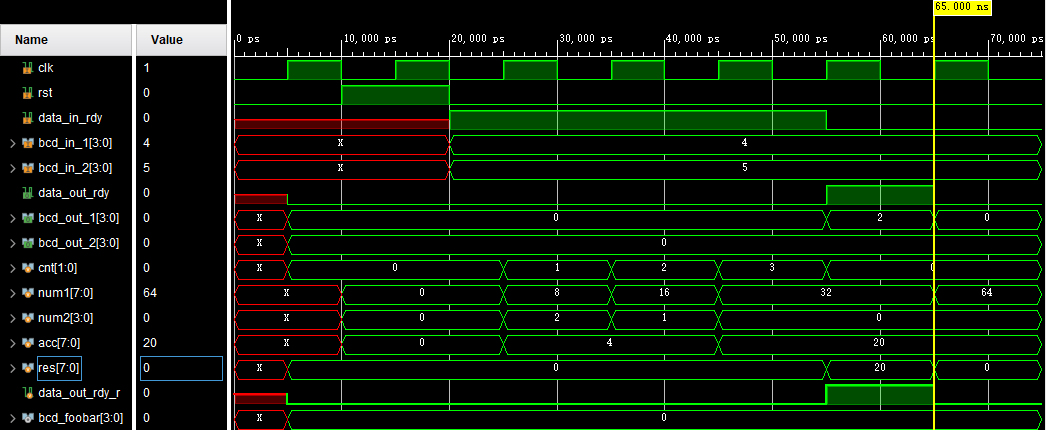
\includegraphics[width=0.7\textwidth]{image/2024-06-20-18-47-58.png}
    \caption{bcd乘法器的仿真结果}
    \label{image_bcd_sim}
\end{figure}
针对BCD乘法器的仿真结果如图\ref{image_bcd_sim}所示, 可以看到随着输入周期的变化, 系统按照时分复用的流程进行计算, 当指定输入数据有效之后, 经过四个周期完成运算, 得到BCD码4和5的乘积结果位20。
\subsection*{提高任务}
\begin{figure}[H]
    \centering
    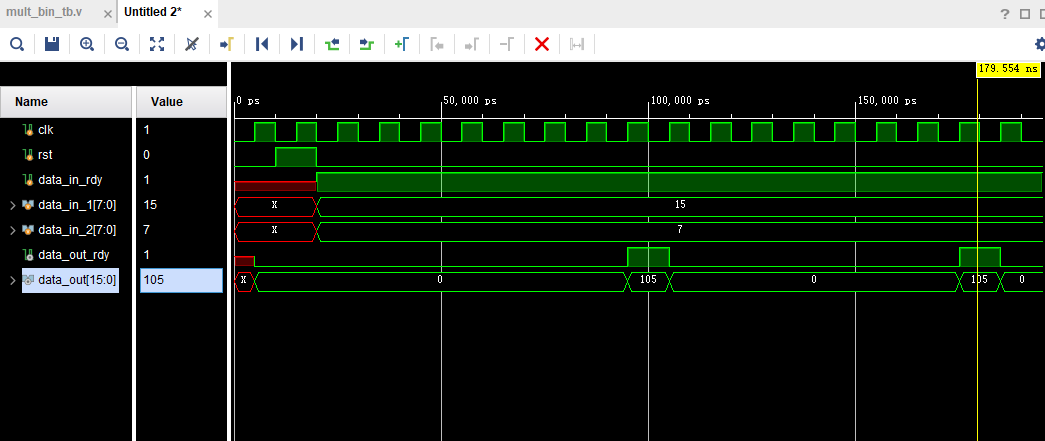
\includegraphics[width=0.7\textwidth]{image/2024-06-24-11-48-32.png}
    \caption{四位二进制乘法的仿真结果}
    \label{image_4bit_sim}
\end{figure}
四位二进制乘法的验证结果如图\ref{image_4bit_sim}所示, 其计算流程与BCD乘法器设计的工作流程一致, 计算结果正确无误。
\subsection*{拓展任务}
\begin{figure}[H]
    \centering
    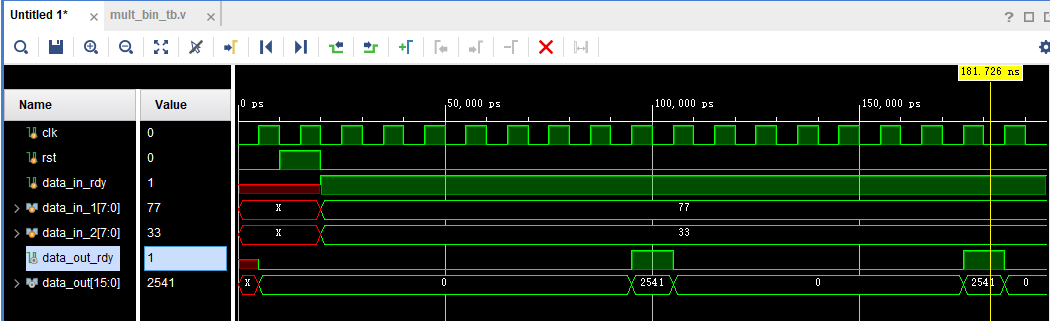
\includegraphics[width=0.7\textwidth]{image/2024-06-24-11-33-41.png}
    \caption{八位二进制乘法的仿真结果}
    \label{image_8bit_sim}
\end{figure}
八位二进制乘法的验证结果如图\ref{image_8bit_sim}所示, 通过4位二进制乘法改变位宽实现,8个周期后完成计算, 计算结果77*33=2541。
% 第四部分
\section*{\fourhao 四、硬件验证结果}
\xiaosihao
\setstretch{1.5}
% 记录加编程器与拨码开关和发光二极管、数码管等的连接情况。记录开发板硬件验证结果,并分析其结果的正确性。
% 按照基础任务、提高任务和拓展任务分别分析
\subsection*{基础任务}
\begin{figure}[H]
    \begin{minipage}[t]{0.45\linewidth}
        \centering
        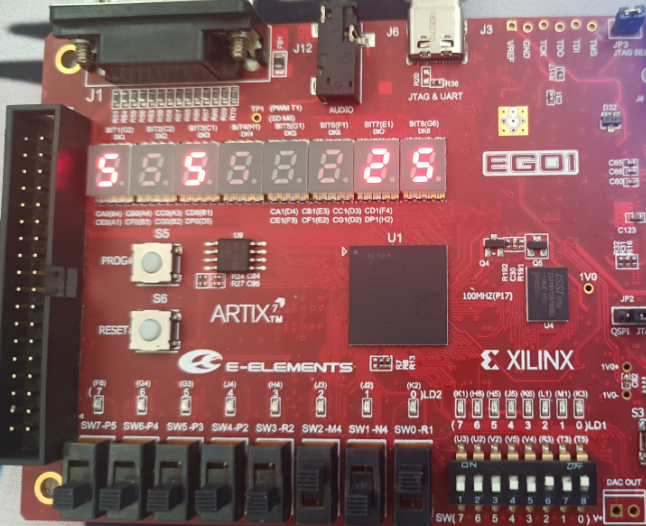
\includegraphics[width=0.7\textwidth]{image/2024-06-24-11-04-31.png}
        \caption{5*5}
        \label{image_verify_1}
    \end{minipage}
    \begin{minipage}[t]{0.45\linewidth}
        \centering
        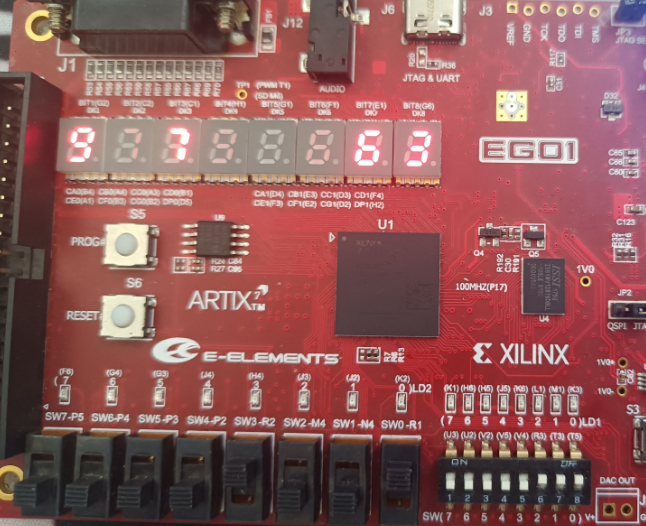
\includegraphics[width=0.7\textwidth]{image/2024-06-24-11-04-56.png}
        \caption{9*7}
        \label{image_verify_2}
    \end{minipage}
\end{figure}
硬件验证结果如图\ref{image_verify_1}和图\ref{image_verify_2}所示, 计算结果正确。
\subsection*{提高任务}
\begin{figure}[H]
    \centering
    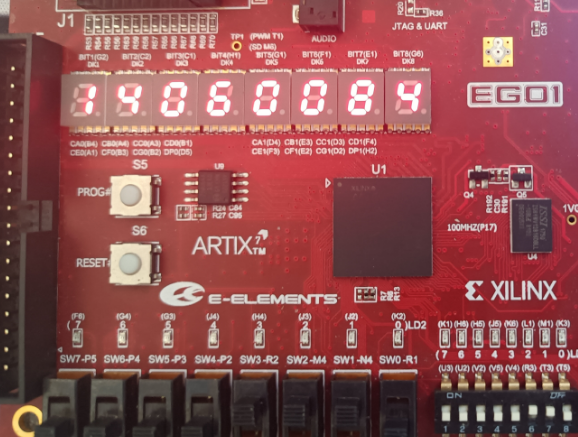
\includegraphics[width=0.3\textwidth]{image/2024-06-24-13-19-25.png}
    \caption{14*6 = 84}
    \label{image_verify_3}
\end{figure}
四位二进制整数乘法的硬件验证结果如图\ref{image_verify_3}, 计算14*6得到结果84, 结果无误。
\subsection*{拓展任务}
\begin{figure}[H]
    \centering
    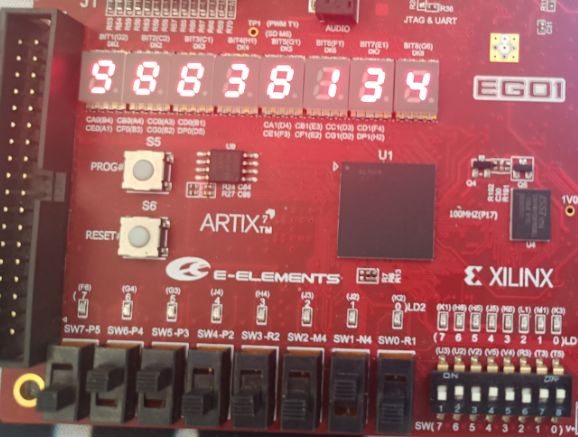
\includegraphics[width=0.3\textwidth]{image/2024-06-24-13-18-41.png}
    \caption{98*83 = 8134}
    \label{image_verify_4}
\end{figure}
8位二进制整数乘法的硬件验证结果如图\ref{image_verify_4}, 计算98*83得到结果8134, 结果无误。
% 第五部分
\section*{\fourhao 五、问题解决}
\xiaosihao
\setstretch{1.5}
% 设计过程中遇到的问题及解决的方法。
\subsection*{加载bit文件后, 数码管显示不正确}
解决: 仿真时主要是对模块进行仿真, top文件中完成的显示和输入没有进行直接的仿真, 导致未发现此次数码管问题, 烧录后数码管仅显示第一位, 起初以为是约束文件出错, 之后通过更改输入的方式发现输出一直, 得到结论:问题出在数码管的部分。\\
首先通过RTL原理图检查问题, 可以直接发现是数码管例化时给的时钟错误, Vivado下的Verilog语法检查器和综合器不会对未经声明而直接用于模块例化的信号产生error, 仅仅会产生warning, 导致此次错误发生。
\subsection*{构建16bit的bin2bcd模块, 不输出}
解决: 图方便直接采用8bit的模块修改得到16bit的模块, 但是输出部分忘了修改, 新模块的输出是bcd\_20bit, 但没有修改原先的语句的左变量:
\begin{lstlisting}[language=Verilog]
assign bcd_12bit = bcd_temp[35-:20];
\end{lstlisting}
但输出的port位bcd\_20bit, 导致错误, 通过查阅资料可以得知, Verilog中支持未声明的线网类型数据, 如wire, 直接使用assign语句声明的同时为其建立组合逻辑关系。
所以综合器没有报错, 最终通过仿真层级关系一层一层检查, 最后发现问题。
\subsection*{修改代码后, 反复重新生成bit文件没有效果}
修改代码后, 首先检查仿真结果, 仿真无误, 但是板上验证结果不对, 推测为Vivado在从综合开始的重新生成bit文件的过程中, 文件被缓存, 更改后的代码没有有效进行综合, 重启vivado后再次进行生成bit文件, 得到正确的结果。
% 第六部分
\section*{\fourhao 六、写出心得体会}
\xiaosihao
\setstretch{1.5}
本次设计过程中通过FPGA完成了简单的算法设计, 也了解到FPGA中设计复杂算法的几种方法, 如果不采用合理的算法和设计结构将导致系统的资源占用过多, 甚至无法实现。
基本的设计流程思路有并行和串行设计, 串行体现的是对资源的时分复用, 而并行就是构建好基础模块后, 重复模块实现复杂算法, 很显然, 为了减少资源的占用, 通常选用串行设计思路。\\
为了解决串行计算中时分复用导致的效率低下, 通常还会采用流水线的设计方式, 将复杂的算法分为不同的处理阶段, 数据串行输入, 同一周期内不同数据进行不同的操作处理, 最终实现的效果就是一个周期可以得到一个计算结果, 在效率和资源上达到一定的平衡。\\
\end{document}
